\chapter{Design of the Controller}
\label{chap:controller}
This chapter is focused on the controller of the Media-Online Management system. The controller consist of a tag reader and power control device which is disgusted in this chapter but when mentioning controller both is implied. \newline
The design and functionality of the prototype controller will be presented in parallel to the designed end product. \newline

\section{Product Design}

There is two devices needed to activate a media from the user to the server as shown in figure \ref{fig:Power&Tagdevice}.


\begin{figure}[h]
	\centering
		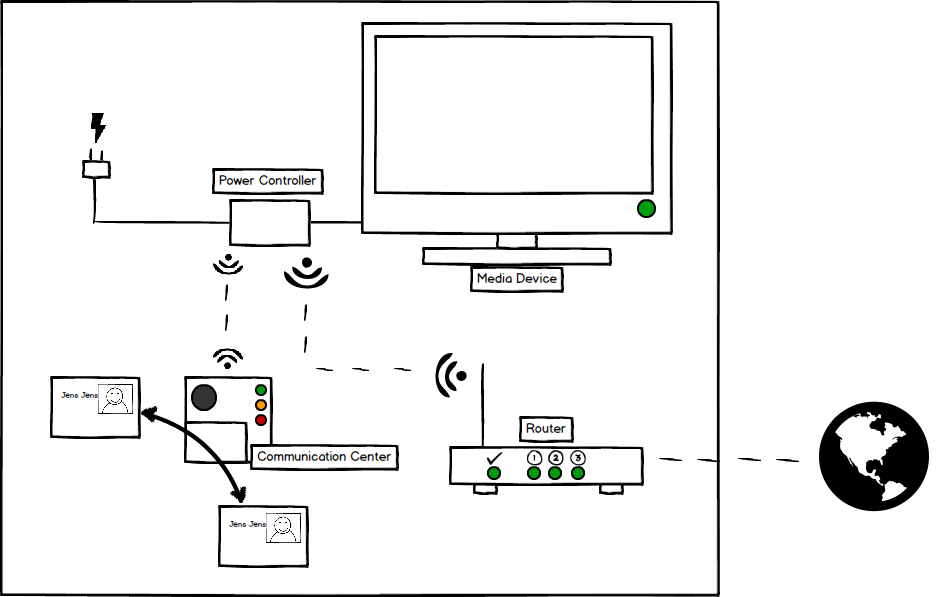
\includegraphics[width=1.00\textwidth]{images/Power&Tagdevice.png}
	\caption{Rich picture for Powercontrol and Tag reader}
	\label{fig:Power&Tagdevice}
\end{figure}

One of them is a small detection device to read the user's tag when swiped over, This device is often placed in the most accessible place. \newline
The other device is a powercontrol device which is located on the powerline to the media device and turns on and off the electricity when needed.\newline
The powercontrol device(PCD) is the brain of the two devices and is therefore to monitor the time usage of the media. It should also communicate with the server and detection device. \newline
The detection device(DD) should also inform the user who is trying to activate a media of whether the activation has been approved or declined by the server.
%The detection device(DD) also works as an information communicator to the user, on the state of the connection to the server about acceptance/decline of log-in. \newline    

\subsection{Senario Design}

The system has been designed on multiple scenarios and the criteria of communication to the server and user. The flow chart \ref{} is an overview of the action and communication the two devices have to give the right permission to user, communicate with the user and server about status, handle disconnection to server and control of user and time usage restrictions.\fixme{sentence makes no sense}\newline

\fixme{indsæt Flowcart af systemet}

To test develop the flowcart of the system is multible usercases constucted.\fixme{sentence makes no sense}\newline


\textbf{Setting up and turning on the system.} \newline
In the final design the PCD will receive the information about the WiFi connection from USB connection.
If the information on the USB is wrong or not received then a restart button is included to redo the procedure.  \newline
The PCD will then connect to the WiFi network and add the controller to the database in his MOM system. If the connection is not found a message is send to the DD. \newline 
DD indicates that there is no connection by showing a constant red light. The communication protocol can be found in the appendix \vref{appen:lights}.\newline When the connection is established then the DD is ready to read user tags.\newline

However, this design will not be implemented in this project. Instead there is a wired connection to the internet and the controller need to be manually added into the database.

\textbf{Detection of connection issues and status changes.} \newline
The connection to the sever is tested by a routine call every five minutes from the PCD to the server. In this call the PCD will receive information on when the media should shutdown based on a rule or the user's remaining time. This insures that if any changes in the remaining time or the rules which will influences when the media should shut down then it will still be handled.
%This insure that there is a connection each five minutes and if any changes in rules or in the time the user may spend on the media. 
In between those calls the PCD will check for a tag from the DD. If the PCD is disconnected from the server that is informed to the DD and to the user.  \newline
	
\textbf{Logon/logoff media divice.} \newline
When a tag is read by the DD the PCD will receive the tag id which is then formed into a log-in message and send to the web servers API. however this is only if no one is all ready logged on the media in the system. The PCD will then get a message about whether the user has permission to use the media from the API. If the user has permission then the PCD should direct power to the media, then save the tag id in local memory and receive the remaining time from the API. The DD should indicate whether the user is approved to use the media.\newline 
To log-off the PCD receive the same tag id that is stored in the local memory. The PCD will then switch off the power to the media and send a log-off message to the API. \newline
If another user wants to take over the usage of the media then the PCD should try to log-in with the new tag. If this is declined then the DD should then signal this and keep the old user logged on. If it is accepted then the server should overwrite the previous user and PCD will receive the information for the new user with out turning the power off and then on again.\newline \fixme{if this has not been included in the implementation then it should be mentioned}


\textbf{Server disconnection under use.} \newline
A disconnection from the server is either found under the regular status call after each five minutes or at a log-on/log-off call. A disconnection will lock the device so only the current user can use the media until the PCD is reconnected with the server. The server discovers the lack of connection when there have not been a status call from the device in five minutes. The disconnection is translated to a log-off the media at the server side. 
The user will not be logged off by the controller but will be able to use his time according to the last status. If the user want to log-off in a period where there is a disconnection a time stamp is saved and will be sent to the server when the connection is reestablished. The media can also first be used again when the connection is reestablished. 
This procedure have the advantage that the user will not have to cut off the media in use if the connection is unstable. The user will also be able to use a another media with connection to the server.
The disadvantage is that the user has the possible to exceed the time restriction if there has been a change in the rules or the user's remaining time. \fixme{if this has not been included in the implementation then it should be mentioned}
		
\section{Prototype Implemtation}
The prototype is designed to prove the concept of the requirements to direct the power to and away from the media, control a tag reader, communicate with the server and it need to be a Embedded system. \newline
To prove the requerments the system the to be able to: 

\begin{itemize}
	\item Read and accept/decline tags in communication with a server though a online connection.
	\item Moniter the connection to server and handele the exseption op disconnected.
	\item Regulate the power to a device recording to senario.
	\item Manage the time usaged and user restigtions. 
	\item Communicat system status to user though LED light indication. 
\end{itemize}




    